% Options for packages loaded elsewhere
\PassOptionsToPackage{unicode}{hyperref}
\PassOptionsToPackage{hyphens}{url}
%
\documentclass[
]{article}
\usepackage{lmodern}
\usepackage{amssymb,amsmath}
\usepackage{ifxetex,ifluatex}
\ifnum 0\ifxetex 1\fi\ifluatex 1\fi=0 % if pdftex
  \usepackage[T1]{fontenc}
  \usepackage[utf8]{inputenc}
  \usepackage{textcomp} % provide euro and other symbols
\else % if luatex or xetex
  \usepackage{unicode-math}
  \defaultfontfeatures{Scale=MatchLowercase}
  \defaultfontfeatures[\rmfamily]{Ligatures=TeX,Scale=1}
\fi
% Use upquote if available, for straight quotes in verbatim environments
\IfFileExists{upquote.sty}{\usepackage{upquote}}{}
\IfFileExists{microtype.sty}{% use microtype if available
  \usepackage[]{microtype}
  \UseMicrotypeSet[protrusion]{basicmath} % disable protrusion for tt fonts
}{}
\makeatletter
\@ifundefined{KOMAClassName}{% if non-KOMA class
  \IfFileExists{parskip.sty}{%
    \usepackage{parskip}
  }{% else
    \setlength{\parindent}{0pt}
    \setlength{\parskip}{6pt plus 2pt minus 1pt}}
}{% if KOMA class
  \KOMAoptions{parskip=half}}
\makeatother
\usepackage{xcolor}
\IfFileExists{xurl.sty}{\usepackage{xurl}}{} % add URL line breaks if available
\IfFileExists{bookmark.sty}{\usepackage{bookmark}}{\usepackage{hyperref}}
\hypersetup{
  pdftitle={STA 325 Final Project},
  pdfauthor={Connie Wu, Jason McEachin, Joe Choo, Scott Heng},
  hidelinks,
  pdfcreator={LaTeX via pandoc}}
\urlstyle{same} % disable monospaced font for URLs
\usepackage[margin=1in]{geometry}
\usepackage{graphicx,grffile}
\makeatletter
\def\maxwidth{\ifdim\Gin@nat@width>\linewidth\linewidth\else\Gin@nat@width\fi}
\def\maxheight{\ifdim\Gin@nat@height>\textheight\textheight\else\Gin@nat@height\fi}
\makeatother
% Scale images if necessary, so that they will not overflow the page
% margins by default, and it is still possible to overwrite the defaults
% using explicit options in \includegraphics[width, height, ...]{}
\setkeys{Gin}{width=\maxwidth,height=\maxheight,keepaspectratio}
% Set default figure placement to htbp
\makeatletter
\def\fps@figure{htbp}
\makeatother
\setlength{\emergencystretch}{3em} % prevent overfull lines
\providecommand{\tightlist}{%
  \setlength{\itemsep}{0pt}\setlength{\parskip}{0pt}}
\setcounter{secnumdepth}{5}

\title{STA 325 Final Project}
\usepackage{etoolbox}
\makeatletter
\providecommand{\subtitle}[1]{% add subtitle to \maketitle
  \apptocmd{\@title}{\par {\large #1 \par}}{}{}
}
\makeatother
\subtitle{Genre Classification using Spotify Data}
\author{Connie Wu, Jason McEachin, Joe Choo, Scott Heng}
\date{11/23/2020}

\begin{document}
\maketitle

\hypertarget{introduction}{%
\section{Introduction}\label{introduction}}

~~~~~~~Cataloging and organizing music is an essential aspect of
collecting and storing music. It allows us not only to identify and
differentiate music, but also allows us to better understand the
evolution of different types of music over periods of time. Genre has
been the main and most efficient mode to categorize different kinds of
music, and genre classification has always been a consistent challenge
due to the complex nature of songs and the difficulty in differentiating
the unique features specific to each genre. In the past, genre
classification was largely performed by using pattern recognition after
breaking the songs down frame by frame, and understanding the elements
of chord progressions and stylistic features of the song {[}1{]}.
However, the rise of big data has allowed us to more efficiently and
accurately extract audio features and consequently automate the arduous
task of classifying songs in particular genres. Genre classification is
not only important in increasing the efficiency of cataloging music
which is relevant to music companies and artists in organizing elements
of their craft, but also for academics who wish to better understand the
evolution of music and particular genres in their research.

~~~~~~~Our study aims to build on modern statistical techniques that
perform genre classification, by predicting the genre of songs based on
multiple audio features each song possesses. Using well-known
classification techniques such as logistic regression and support vector
machines (SVM), we leverage the substantial capacity of modern computing
to perform such statistical modeling on a large dataset of songs and
various audio features taken from Spotify, and compare the performance
of both classification techniques so as to evaluate their predictive
accuracies, strengths and weaknesses of using either approach for genre
classification. Using both methods to perform multi-group
classification, this study aims to comprehensively and comparatively
evaluate the effectiveness of both statistical methods with respect to
music analytics.

~~~~~~~Our paper is organized holistically and with simplicity to
provide a comprehensive report on genre classification, starting with
introducing research goals and providing the background motivations for
the study. In Section 2, we provide a a description of the data as well
as extensive exploratory data analysis which will motivate some design
decisions during our statistical modeling. Section 3 describes our
methodology with respect to implementing logistic regression and support
vector machines for predicting genres of songs, structured with
multi-group classification. In Section 4, we discuss our models' results
as well as model diagnostics to evaluate the accuracy of each of the
models' fit, and relate our results to relevant parties that will use
genre classification. Finally in section 5, we consolidate our findings
and conclude our study with its strengths and its limitations.

\hypertarget{data}{%
\section{Data}\label{data}}

~~~~~~~Our data was taken from Spotify's API, that draws from its large
database of songs and their respective audio features. The data set was
consolidated and released on kaggle, containing 232,725 tracks across 26
genres {[}2{]}. Each data point represents a song along with its tagged
genre and various audio attributes such as tempo, key, danceability,
valence, acousticness etc. For a detailed description of each feature,
please refer to Table 2.1.

\begin{table}[!h]

\caption{\label{tab:unnamed-chunk-4}Table 2.1 Descriptions of data set variables}
\centering
\fontsize{9}{11}\selectfont
\begin{tabular}[t]{rl>{\raggedright\arraybackslash}p{10cm}l}
\toprule
Col & Column.Name & Description & Value\\
\midrule
1 & acousticness & A measure of degree of how acousitc a track is. 1.0 is most acoustic & float (0.0-1.0)\\
2 & danceability & A measure  based on a combination of music elements including tempo, rhythm stability, beat strength, and overall regularity. A value of 1.0 is most danceable & float (0.0-1.0)\\
3 & duration\_ms & Duration of the track in milliseconds & integer\\
4 & energy & A perceptual measure of intensity and activity attributing dynamic range, perceived loudness, timbre, onset rate, and general entropy. & float (0.0-1.0)\\
5 & instrumentalness & A measure of the presence of vocals, rap or spoken word. The higher the value, the greater likelihood the track contains no vocal content. & float (0.0-1.0)\\
\addlinespace
6 & key & Integers that  map to pitches using the standard pitch class (C=1, C\#=2 …) & integer\\
7 & liveness & A measure that detects the presence of an audience in the recording.  A value above 0.8 provides strong likelihood that the track is live & float (0.0-1.0)\\
8 & loudness & The overall loudness of a track in decibels (dB). Loudness values are averaged across the entire track.  Values typical range between -60 and 0 db & float (0.0-1.0)\\
9 & speechiness & A measure that detects the presence of spoken words in a track & float (0.0-1.0)\\
10 & popularity & A measure of the song's popularity, calculated by considering the track's total number of plays and how recent those plays are. & integer (0-100)\\
\addlinespace
11 & tempo & The overall estimated tempo of a track in beats per minute (BPM)- the speed or pace of a given piece and derives directly from the average beat duration. & float (0.0-1.0)\\
12 & valence & A measure  describing the musical positiveness conveyed by a track. Tracks with high valence sound more positive (e.g. happy, cheerful, euphoric) & float (0.0-1.0)\\
13 & year & Year that the track was released & integer\\
14 & mode & Modality of the track (1=Major, 0=Minor) & integer\\
15 & name & Name of track & string\\
\addlinespace
16 & genres & Genres associated with the track's artist(s) & array\\
17 & artist & Name of the track's main artist & string\\
\bottomrule
\end{tabular}
\end{table}

~~~~~~~Before proceeding further, we performed some data cleaning.
Firstly, we eliminated any observations that had the genre `acapella',
because it was a duplicate of a full song already included in the
dataset and it had only 119 observations. We also removed any
observations with `Comedy' as they are lengthy tracks of spoken word by
comedians, and we considered them not to be actual music. We also got
rid of Children's Music due to faulty labeling, and Reggae because it is
extremely similar to Ska.

\hypertarget{exploratory-data-analysis}{%
\subsection{Exploratory Data Analysis}\label{exploratory-data-analysis}}

~~~~~~~We began our exploratory data analysis to better understand the
composition of our dataset. Starting with understanding the breakdown of
genres, we see from Fig 1 that there is a good amount of observations
for each group (\textgreater6000), which tells us that there will be
enough observations to classify each of our 22 genres, and techniques
like bootstrapping or strategies to deal with limited data do not need
to be considered.

\begin{figure}
\centering
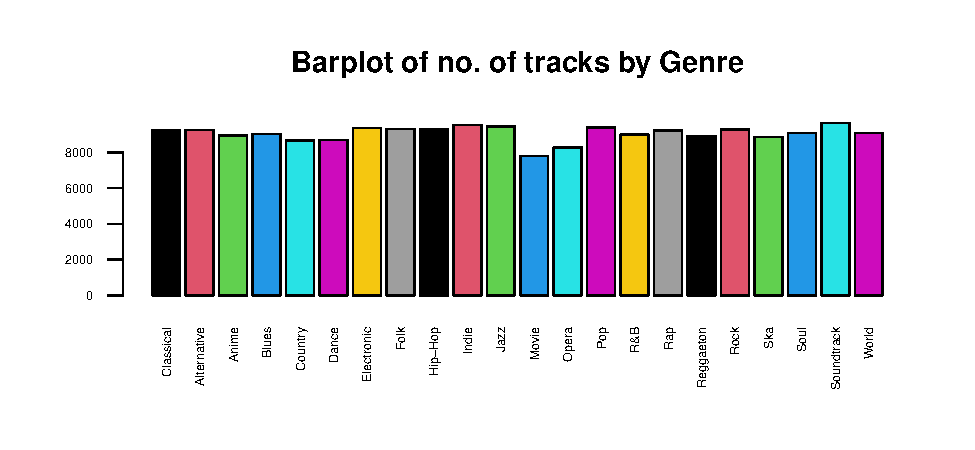
\includegraphics{write-up_files/figure-latex/count occurrences-1.pdf}
\caption{Count of tracks per Genre}
\end{figure}

~~~~~~~We then looked to understand the compositions of audio features
based on genres, by generating density plots for each audio feature. Fig
1.2 shows the density plots of 6 audio features, and we can observe that
although for features such as danceability, energy and tempo, each genre
has a relatively distinctive density plot while for features such as
liveness, loudness and valence, the densities are much hard to
differentiate. Please refer to the appendix for density plots for the
remaining audio features.

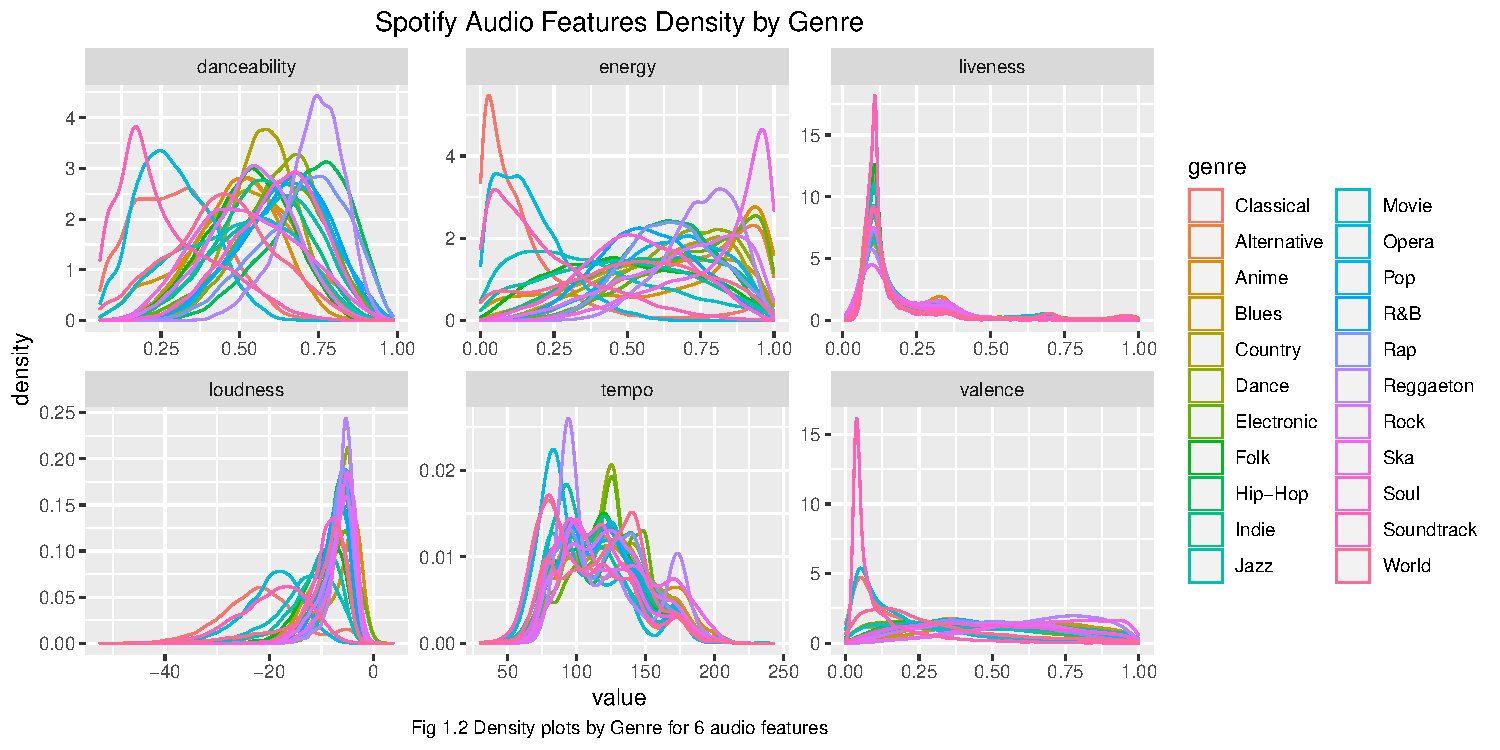
\includegraphics{write-up_files/figure-latex/unnamed-chunk-5-1.pdf}

\hypertarget{methodology}{%
\section{Methodology}\label{methodology}}

\hypertarget{binary-and-multinomial-logistic-regression}{%
\subsection{Binary and Multinomial Logistic
Regression}\label{binary-and-multinomial-logistic-regression}}

~~~~~~~The first of our two classification techniques we chose to model
to predict genres is logistic regression. Logistic regression is
appropriately used in cases when the dependent variable is categorical,
which in our study's dependent variable being genre. It is not only
computationally efficient but is produces results that are easy to
interpret. As our EDA has shown a substantial amount of observations
(\textgreater6000 for each genre) that are much more than the number of
features (\textasciitilde13), there is a high level of confidence that
overfitting will not occur, however more comprehensive model diagnostics
will be performed and described in the later sections. Logistic
Regression is usually performed when the dependent variable is
dichotomous, meaning that the model can perform predictive
classification over 2 genres. Also known as the log-odds model, logistic
regression can be written mathematically as:

\[
l = \text{log} (\frac{p}{1-p}) = \beta_0 + \sum_{i=1}^{13}\beta_i x_i
\] where \(l\) is the log-odds and \(p\) = \(P(Y=1)\) is the probability
of the observation being classified as one group labelled \(Y=1\),
\(\beta_0\) is the intercept and \(\beta_i\) are the coefficients of the
13 predictors, in our study being audio features, represented as
\(x_i\).

~~~~~~~While logistic regression can be used for binary classification
between two genres, this approach can be easily expanded to perform
multi-group classification. The extension appropriate for our study is
called multinomial logistic regression, which is similar to binary
logistic regression, with the exception of having J-1 equations instead
of one, J being the number of categories encompassed in the model. This
can be written in mathematical notation as:

\[
l = log( \frac{\pi_{ij}}{\pi_{iJ}} )= \beta_0 + \mathbf{x_i} \boldsymbol{\beta_j}
\]

where \(\boldsymbol{\beta_j}\) is a vector of regression coefficients,
similar to \(\mathbf{x_i}\) being a vector of predictors. This produces
\(J-1\) multinomial logit equations that contrast each of the
categories, compared to binary logistic regression that contrasts
between successes \(Y=1\) and failures \(Y=0\).

\hypertarget{support-vector-machine-svm}{%
\subsection{Support Vector Machine
(SVM)}\label{support-vector-machine-svm}}

~~~~~~~The second classification technique is a supervised machine
learning model, chosen appropriately as our data is completely labeled.
SVM performs classification by generating one or multiple hyperplanes
with \(p\) dimensions, \(p\) being the number of predictors included in
the model. A function is intuitively set to divide the points between
two classes, forming what is known as a separating hyperplane. Among the
separating hyperplanes created, the one making the largest margin
between the two classes is chosen as the optimal model and is used for
predictions.

~~~~~~~For both the multinomial logistic and SVM models, we will only be
using the top 5 genres, as more genres significantly decreases the
predictive accuracy of the multinomial model. These top 5 genres are
Electronic, Indie, Jazz, Pop, and Soundtrack.

\hypertarget{results}{%
\section{Results}\label{results}}

\hypertarget{multinomial-logistic-regression}{%
\subsection{Multinomial Logistic
Regression}\label{multinomial-logistic-regression}}

~~~~~~~To obtain this model, we put in all variables other than
``genre'' into a multinomial logistic regression model and performed
backwards step-wise selection. All variables were chosen except for
\texttt{liveness}. We decided not to explore any interaction terms, as
we believe that this would negatively affect the interpretability of our
model.

~~~~~~~The coefficients of our final model can be found in the Appendix.
It is important to note that the ``Electronic'' genre is the baseline
genre in this model. We can see that the log-odds of a song being Pop
versus Electronic when all variables have a value of 0 is -13.1, whereas
the log-odds of a song being Soundtrack versus Electronic when all
variables have a value of 0 is 7.83. This means that when all variables
are 0, the odds are high of the song being in the Soundtrack genre
vs.~Electronic, whereas the odds are very low of the song being in the
Pop genre vs.~Electronic.

~~~~~~~One variable that had a broad range of coefficient values among
all the genres was danceability. We can see that all coefficient values
are negative, meaning that with each 1 unit increase in danceability,
holding all else constant, the log-odds of a song being any of the four
genres other than Electronic vs.~Electronic decreases by some amount.
For example, with a 1 unit increase in danceability, holding all else
constant, the log-odds of a song being Soundtrack vs.~Electronic
decreases by -11.9, whereas it decreases by -3.04 for Pop. This means
that Electronic typically has the highest danceability rating out of the
other 4 genres, with Soundtrack typically having the lowest danceability
rating.

~~~~~~~Another interesting variable that we can interpret is popularity.
We can see that all coefficient values are positive except for
Soundtrack's, meaning that with each 1 unit increase in popularity,
holding all else constant, the log-odds of a song being Indie, Jazz, or
Pop vs.~Electronic increases by some amount, whereas the log-odds of a
song being Soundtrack vs.~Electronic decreases by some amount. More
specifically, with a 1 unit increase in popularity, holding all else
constant, the log-odds of a song being Soundtrack vs.~Electronic
decreases by -0.05, whereas it increases by 0.39 for Pop. In fact,
because Pop's coefficient for popularity is the highest out the 4, we
can see that Pop typically has the highest popularity, which makes sense
because Pop music is typically what is played on mainstream radio
stations. On the other hand, we can see that Soundtrack typically has
the lowest popularity out of the 5 genres.

\hypertarget{model-validation-and-diagnostics}{%
\subsubsection{Model Validation and
Diagnostics}\label{model-validation-and-diagnostics}}

~~~~~~~We performed 5-fold cross-validation on our model, the results of
which can be found in our Appendix. We partitioned the data into 90\%
for the training set and 10\% for the test set. We then partitioned the
training set 5 more times to obtain several estimates for 5-fold
cross-validation. We averaged these estimates and obtained 0.747, or
74.7\% accuracy. Then, we trained the model on the whole training set
(90\% of the data) and predicted on the testing set (10\% of the data)
and obtained a prediction accuracy of 74.2\%. This is relatively
accurate and all of the estimates are around the same, indicating that
our model is not overfitting the training set.

\begin{figure}

{\centering 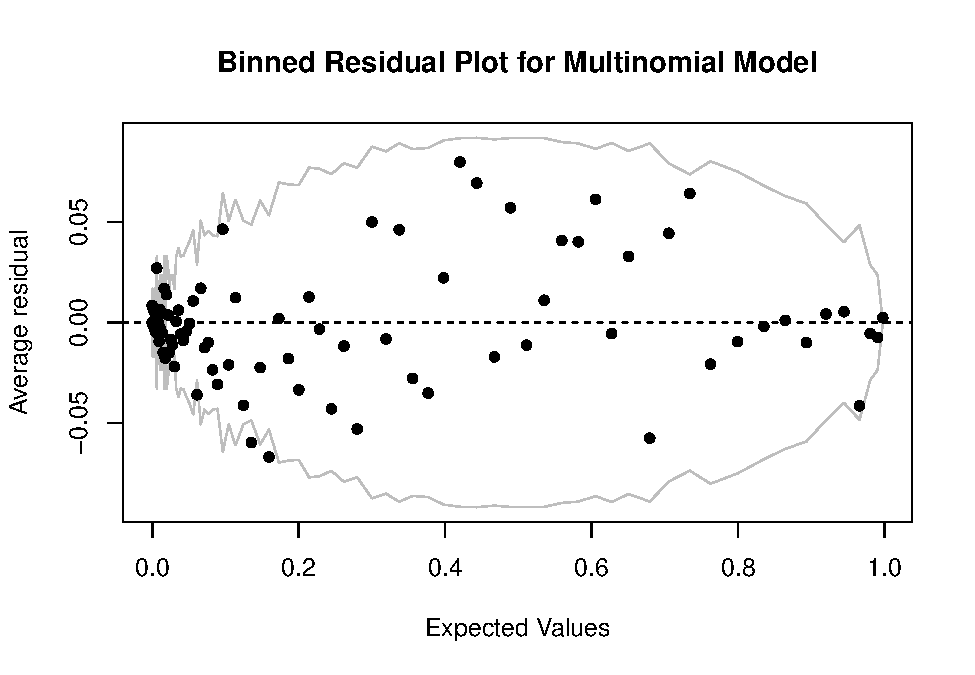
\includegraphics[width=0.8\linewidth]{write-up_files/figure-latex/unnamed-chunk-7-1} 

}

\caption{Binned Residual Plot for Multinomial Model}\label{fig:unnamed-chunk-7}
\end{figure}

~~~~~~~From this residual plot, it appears that less than 5\% of the
observations lie outside of the gray lines, which represent the ±2
standard error bands. Additionally, the residuals appear to be mostly
randomly scattered, although a large amount of the residuals are crowded
at the left end of the plot. Overall, we can see that our model suits
the data relatively well.

\hypertarget{svm}{%
\subsection{SVM}\label{svm}}

~~~~~~~The SVM model was fit using the variables chosen from backward
selection as in the case for Multinomial Logistic Regression to keep
consistent. As a result, the only variable not chosen in the final model
was that of liveliness. It is important to note that we using a radial
kernel, which is better for creating separation for non-linear
relationships. This made sense because from the Exploratory Data
Analysis section, it can be seen that linear hyperplanes could not be
drawn to cleanly separate genres from each other based on the
predictors.

~~~~~~~The output from the SVM model indicates that from our training
dataset tells us there are 1982 support vectors. We fit the model with a
relatively low cost gives that was rather robust. We obtained the
optimal cost of 5 for our model using cross-validation through the
function \texttt{tune()} in R. The number of support vectors given the
training data follows from our choice of C as we increase C there are
fewer support fewer vectors. Further, as shown in the resulting table,
76\% of our training observations were correctly classified.

\hypertarget{conclusions}{%
\section{Conclusions}\label{conclusions}}

~~~~~~~Perhaps the largest takeaway of this project is seeing how
Multinomial Logistic Regression (MLR) and Support Vector Machines (SVM)
are related to each other, as well as limitation of use for each model.
The test accuracy for MLR and SVM were 74.2\% and 76\% respectively, and
although SVM is more efficient and accurate, we sacrifice
interpretability as to how each predictor may affect the likelihood of a
particular genre being correctly classfied. With more knowledge about
the distribution of our data through empirical and EDA observations, we
determined that SVM with a radial kernal was most appropriate for
predicting our data. This was because natural clusters (not linear
separations) formed depending on the genres' predictors. These
separations were better identified through SVM which may account for the
slightly higher test accuracy.

~~~~~~~A limitation/obstacle in the course of this case study was
choosing how many different genres to consider in our models.
Unfortunately, we had to immediately rule out using all/most of the
cleaned 22 genres to choose from, due to computational limits in our
local machines when running a MLR. Additionally, in the scope of
Spotify's mission to provide popular songs to stream, analyze, and
curate playlists from, it made sense to look at a ``Top 10'' genres,
which ruled out more niche genres such as Anime, Ska, and Blue. However,
due to overlap in many of the different indicators (many of which were
scaled in a range of 0-1 as determined by Spotify), predictive power was
lacking so we decided to narrow the field further and use the ``Top 5''
genres. Therefore to create meaningful models in context of usefulness
for Spotify and to explore and analyze the nuances of MLR and SVM
largely drove this project.

~~~~~~~In terms of impacts, having a high level of accuracy is important
so Spotify can classify, organize, and ultimately recommend specific
genres and songs to its users. While we only looked at the Top 5 genres,
grouping models into bins of 5 might be an effective way to maintain
fairly high predictability as well as manage computational limits. For
example, in future analysis, we can take the Top 6-10 genres, the Top
11-15 genres, and the Top 16-22 genres and apply it to unknown
genre-classified songs. This would allow for several possible
predictions to which ultimately the highest likelihood for example could
be chosen to finally label and predict the song's genre. This
segmentation eases computational load and maintains higher accuracy as
the possible outcomes are more clear to predict instead of a particular
genre being among a crowd of other 21 genres with similar key
predictors. In order to improve the results in future findings, perhaps
more predictor variables would be useful. The indicators as given by
Spotify reflect the aggregate of a particular song and does not account
for, say: chord progression; change of keys, tempo, or loudness
throughout the course of a song; and thematic or descriptive traits that
might be indicative of a genre.

\hypertarget{works-cited}{%
\section{Works Cited}\label{works-cited}}

{[}1{]} C.N. Silla Jr., A.L. Koerich, C.A.A. Kaestner A machine learning
approach to automatic music genre classification J Braz Comput Soc, 14
(3) (2008)

{[}2{]}
\url{https://www.kaggle.com/zaheenhamidani/ultimate-spotify-tracks-db}

\hypertarget{appendix}{%
\section{Appendix}\label{appendix}}

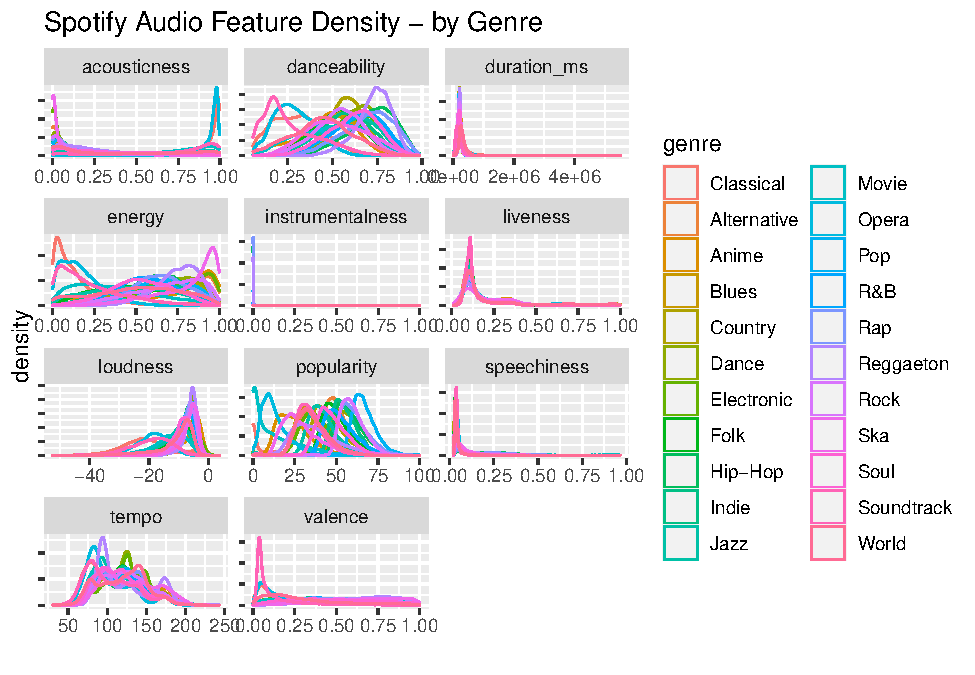
\includegraphics{write-up_files/figure-latex/unnamed-chunk-8-1.pdf}

\hypertarget{eda}{%
\subsection{EDA}\label{eda}}

\begin{center}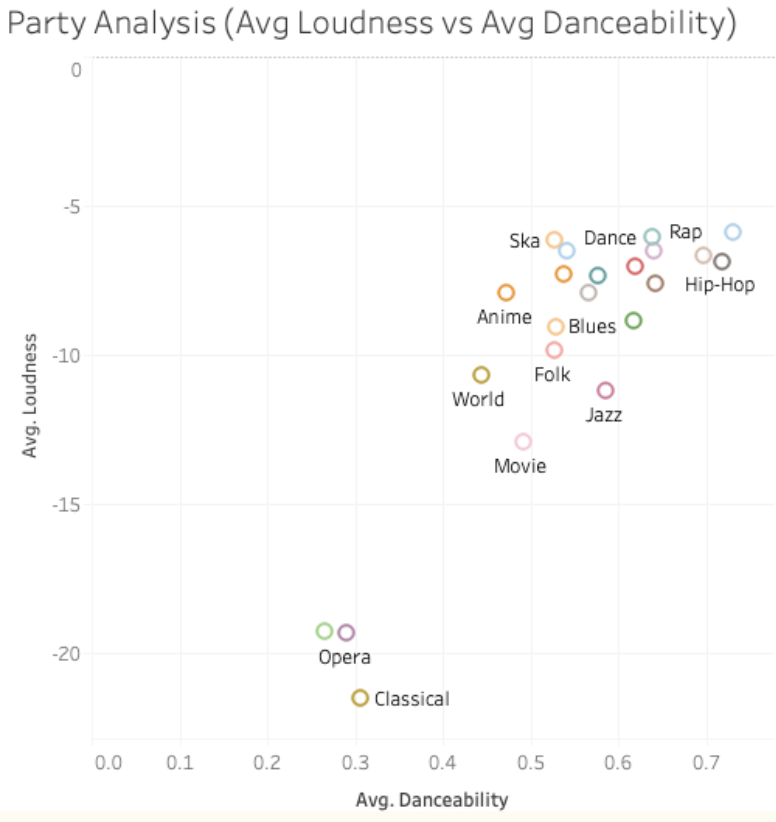
\includegraphics[width=0.7\linewidth]{Screen Shot 2020-11-23 at 11.34.18 PM} \end{center}

\begin{center}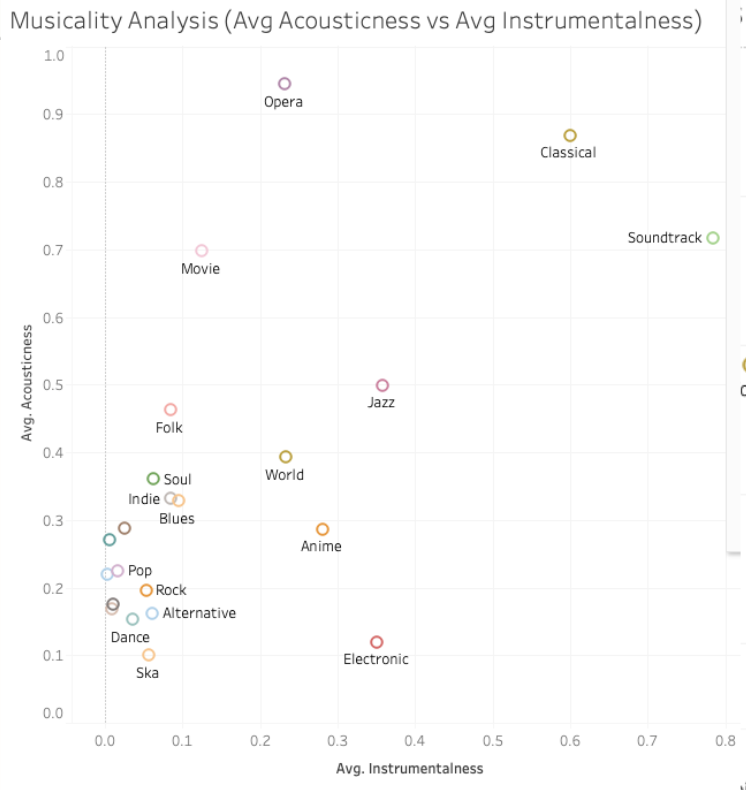
\includegraphics[width=0.7\linewidth]{Screen Shot 2020-11-23 at 11.34.30 PM} \end{center}

\begin{center}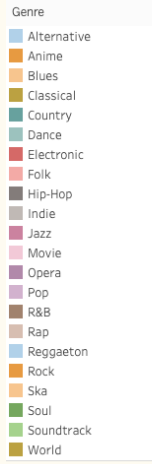
\includegraphics[width=0.7\linewidth]{Screen Shot 2020-11-23 at 11.34.46 PM} \end{center}

\hypertarget{multinomial-logistic-regression-model-coefficients}{%
\subsection{Multinomial Logistic Regression Model
Coefficients}\label{multinomial-logistic-regression-model-coefficients}}

\begin{verbatim}
## Call:
## multinom(formula = genre ~ popularity + acousticness + danceability + 
##     duration_ms + energy + instrumentalness + loudness + speechiness + 
##     tempo + valence, data = train5)
## 
## Coefficients:
##            (Intercept)  popularity acousticness danceability   duration_ms
## Indie       -0.1621498  0.19073438     1.739542    -5.187256 -4.836917e-06
## Jazz         4.1162811  0.02743972     1.853528    -4.972872  2.714906e-07
## Pop        -13.0611427  0.39393495     1.480342    -3.045157 -5.347594e-06
## Soundtrack   7.8328288 -0.04928726     1.397582   -11.878656 -7.318617e-06
##               energy instrumentalness    loudness speechiness        tempo
## Indie      -5.378662      -2.02572993  0.18382104  -2.7388335 -0.003380295
## Jazz       -6.066768      -0.04108421  0.02128958  -1.1968175 -0.007950603
## Pop        -5.429040      -2.24413299  0.29988810   0.1732901 -0.002966148
## Soundtrack -3.117103       1.99873541 -0.17905762  -5.2492121 -0.007306684
##              valence
## Indie      2.1337518
## Jazz       4.7591732
## Pop        2.0413673
## Soundtrack 0.9078647
## 
## Std. Errors:
##             (Intercept)   popularity acousticness danceability  duration_ms
## Indie      4.529557e-06 0.0002508127 1.093684e-06 2.713171e-06 6.368455e-07
## Jazz       5.816945e-06 0.0002475939 2.737776e-06 3.370431e-06 4.213654e-07
## Pop        2.345541e-06 0.0001441456 3.006941e-07 1.496770e-06 5.936776e-07
## Soundtrack 2.496237e-06 0.0000954572 1.698863e-06 1.201521e-06 4.791655e-07
##                  energy instrumentalness     loudness  speechiness        tempo
## Indie      3.212523e-06     4.007419e-07 2.950040e-05 5.152618e-07 0.0009973387
## Jazz       2.893413e-06     1.765160e-06 6.112257e-05 5.098701e-07 0.0008777136
## Pop        1.767150e-06     8.056668e-08 1.381450e-05 2.604704e-07 0.0005750063
## Soundtrack 8.518546e-07     1.370789e-06 3.730441e-05 1.580633e-07 0.0003820034
##                 valence
## Indie      2.777095e-06
## Jazz       2.935101e-06
## Pop        1.719798e-06
## Soundtrack 8.776291e-07
## 
## Residual Deviance: 3703.08 
## AIC: 3791.08
\end{verbatim}

\hypertarget{multinomial-cross-validation-results}{%
\subsubsection{Multinomial Cross Validation
Results}\label{multinomial-cross-validation-results}}

\begin{verbatim}
## # weights:  60 (44 variable)
## initial  value 9766.069253 
## iter  10 value 7094.303915
## iter  20 value 5222.951456
## iter  30 value 4379.187798
## iter  40 value 3929.692676
## iter  50 value 3882.967002
## iter  60 value 3881.528720
## final  value 3881.526834 
## converged
## # weights:  60 (44 variable)
## initial  value 9766.069253 
## iter  10 value 7054.856554
## iter  20 value 5356.808212
## iter  30 value 4415.294131
## iter  40 value 3948.612821
## iter  50 value 3893.270773
## iter  60 value 3892.013171
## final  value 3892.009087 
## converged
## # weights:  60 (44 variable)
## initial  value 9766.069253 
## iter  10 value 6882.799927
## iter  20 value 5125.796361
## iter  30 value 4357.108660
## iter  40 value 3922.084565
## iter  50 value 3874.988549
## iter  60 value 3874.016720
## final  value 3874.014448 
## converged
## # weights:  60 (44 variable)
## initial  value 9766.069253 
## iter  10 value 7006.459608
## iter  20 value 5627.407997
## iter  30 value 4338.487811
## iter  40 value 3918.320191
## iter  50 value 3837.148379
## iter  60 value 3835.593484
## final  value 3835.591811 
## converged
## # weights:  60 (44 variable)
## initial  value 9766.069253 
## iter  10 value 6843.570171
## iter  20 value 5249.695759
## iter  30 value 4405.019868
## iter  40 value 3961.497982
## iter  50 value 3908.506751
## iter  60 value 3906.700836
## final  value 3906.699292 
## converged
\end{verbatim}

\begin{verbatim}
## [1] 0.7369809 0.7475280 0.7481872 0.7574160 0.7468688
\end{verbatim}

\begin{verbatim}
## [1] 0.7473962
\end{verbatim}

\begin{verbatim}
## # weights:  60 (44 variable)
## initial  value 12207.586566 
## iter  10 value 8738.454259
## iter  20 value 6353.506944
## iter  30 value 5384.023406
## iter  40 value 4925.452171
## iter  50 value 4854.955465
## iter  60 value 4853.215507
## final  value 4853.212273 
## converged
\end{verbatim}

\begin{verbatim}
##             
## preds        Electronic Indie Jazz Pop Soundtrack
##   Electronic        270    22   68   2         16
##   Indie              38   250   45  65          6
##   Jazz               46    28  238   1         21
##   Pop                 9    78    2 306          0
##   Soundtrack         12     4   24   1        343
\end{verbatim}

\begin{verbatim}
## [1] 0.7424802
\end{verbatim}

\hypertarget{support-vector-machine-model}{%
\subsection{Support Vector Machine
Model}\label{support-vector-machine-model}}

\begin{verbatim}
## 
## Call:
## svm(formula = genre ~ . - liveness, data = train5, cost = 5, kernel = "radial")
## 
## 
## Parameters:
##    SVM-Type:  C-classification 
##  SVM-Kernel:  radial 
##        cost:  5 
## 
## Number of Support Vectors:  1624
## 
##  ( 326 162 452 271 413 )
## 
## 
## Number of Classes:  5 
## 
## Levels: 
##  Electronic Indie Jazz Pop Soundtrack
\end{verbatim}

\begin{verbatim}
## [1] 76.01
\end{verbatim}

\begin{verbatim}
## 
## Parameter tuning of 'svm':
## 
## - sampling method: 10-fold cross validation 
## 
## - best parameters:
##  cost
##     1
## 
## - best performance: 0.2457685 
## 
## - Detailed performance results:
##    cost     error dispersion
## 1 1e-03 0.8002805 0.01545892
## 2 1e-02 0.3948653 0.04200715
## 3 1e-01 0.2679145 0.02216319
## 4 1e+00 0.2457685 0.02597425
## 5 5e+00 0.2499914 0.02403705
## 6 1e+01 0.2570262 0.02320843
## 7 1e+02 0.2985137 0.02415483
\end{verbatim}

\end{document}
